\usetikzlibrary{automata, positioning}

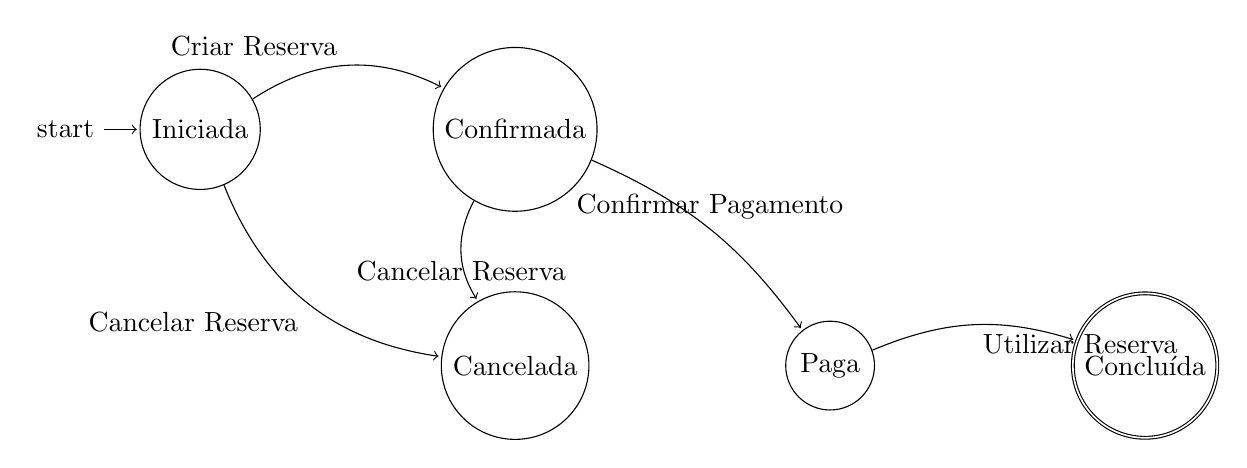
\begin{tikzpicture}[shorten >=1pt, node distance=3cm and 4cm, on grid, auto]
   % Definição dos estados
   \node[state, initial] (iniciada)   {Iniciada};
   \node[state] (confirmada) [right=of iniciada] {Confirmada};
   \node[state] (paga) [below right=of confirmada] {Paga};
   \node[state] (cancelada) [below=of confirmada] {Cancelada};
   \node[state, accepting] (concluida) [right=of paga] {Concluída};

   % Definição das transições
   \path[->]
    (iniciada) edge [bend left] node {Criar Reserva} (confirmada)
               edge [bend right] node [below left] {Cancelar Reserva} (cancelada)
    (confirmada) edge [bend left=15] node [above] {Confirmar Pagamento} (paga)
                 edge [bend right] node [below] {Cancelar Reserva} (cancelada)
    (paga) edge [bend left=20] node [below right] {Utilizar Reserva} (concluida);
\end{tikzpicture}